% This file was created by matlab2tikz.
% Minimal pgfplots version: 1.3
%
%The latest updates can be retrieved from
%  http://www.mathworks.com/matlabcentral/fileexchange/22022-matlab2tikz
%where you can also make suggestions and rate matlab2tikz.
%


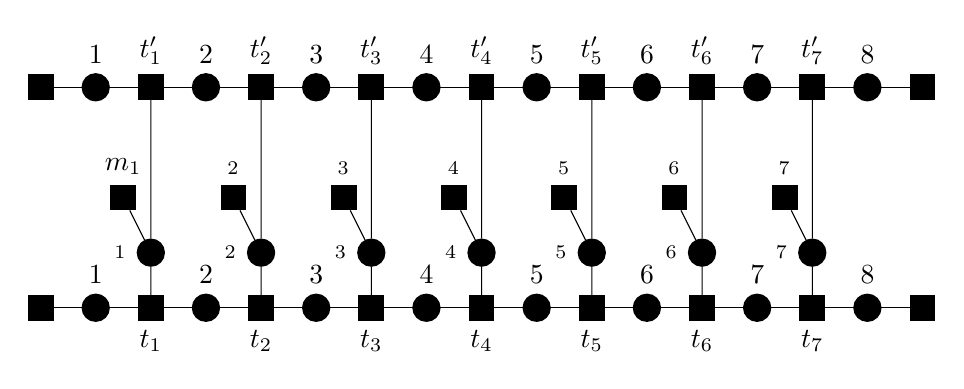
\begin{tikzpicture}[scale=0.35]
\tikzstyle{factor}=[rectangle,minimum size = 3mm, thick, draw =black,fill=black]
\tikzstyle{var}=[circle,minimum size = 3mm, thick, draw =black,fill=black]
\tikzstyle{second}=[circle, minimum size = 5mm, thick]
\tikzstyle{box}=[rectangle, draw=black!100]
\tikzstyle{connect}=[-latex, thick]

	   \pgfmathsetmacro{\posh}{-1};	
	   
	\node[factor] (tphi0) at (0,0) [label=below:{}]{};
	\node[var] (phi0) at (2,0) [label=above:{$\st{1}$}]{};
	\node[factor] (tphi1) at (4,0) [label=below:{$t_1$}]{};
	\node[var] (s0) at (4,2) [label=left:{$\x_1$}]{};
	\node[factor] (fs0) at (\posh+4,4) [label=above:{$\p{m_1}$}]{};
	
	\node[var] (phi1) at (6,0) [label=above:{$\st{2}$}]{};
	\node[factor] (tphi2) at (8,0) [label=below:{$t_2$}]{};
	\node[var] (s1) at (8,2) [label=left:{$\x_2$}]{};
	\node[factor] (fs1) at (\posh+8,4) [label=above:{$\p{\x_2}$}]{};	

	
	\node[var] (phi2) at (10,0) [label=above:{$\st{3}$}]{};
	\node[factor] (tphi3) at (12,0) [label=below:{$t_3$}]{};
		\node[var] (s2) at (12,2) [label=left:{$\x_3$}]{};
	\node[factor] (fs2) at (\posh+12,4) [label=above:{$\p{\x_3}$}]{};		
	
	\node[var] (phi3) at (14,0) [label=above:{$\st{4}$}]{};
	\node[factor] (tphi4) at (16,0) [label=below:{$t_4$}]{};
	\node[var] (s3) at (16,2) [label=left:{$\x_4$}]{};	
	\node[factor] (fs3) at (\posh+16,4) [label=above:{$\p{\x_4}$}]{};
	
	\node[var] (phi4) at (18,0) [label=above:{$\st{5}$}]{};
	\node[factor] (tphi5) at (20,0) [label=below:{$t_5$}]{};
	\node[var] (s4) at (20,2) [label=left:{$\x_5$}]{};	
	\node[factor] (fs4) at (\posh+20,4) [label=above:{$\p{\x_5}$}]{};	
	
	\node[factor] (fs5) at (\posh+24,4) [label=above:{$\p{\x_6}$}]{};	
	\node[var] (s5) at (24,2) [label=left:{$\x_6$}]{};	
	\node[var] (phi5) at (22,0) [label=above:{$\st{6}$}]{};
	\node[factor] (tphi6) at (24,0) [label=below:{$t_6$}]{};	
	
	\node[factor] (fs6) at (\posh+28,4) [label=above:{$\p{\x_7}$}]{};	
	\node[var] (s6) at (28,2) [label=left:{$\x_7$}]{};	
	\node[var] (phi6) at (26,0) [label=above:{$\st{7}$}]{};
	\node[factor] (tphi7) at (28,0) [label=below:{$t_7$}]{};
	\node[var] (phi7) at (30,0) [label=above:{$\st{8}$}]{};
	\node[factor] (tphi8) at (32,0) [label=below:{}]{};
	
	\path
		(tphi0) edge [] (tphi8)
		(fs0) edge [] (s0)
		(s0) edge [] (tphi1)
		(fs1) edge [] (s1)
		(s1) edge [] (tphi2)
		(fs2) edge [] (s2)
		(s2) edge [] (tphi3)
		(fs3) edge [] (s3)
		(s3) edge [] (tphi4)		
		(fs4) edge [] (s4)
		(s4) edge [] (tphi5)
		(fs5) edge [] (s5)
		(s5) edge [] (tphi6)	
		(fs6) edge [] (s6)
		(s6) edge [] (tphi7);	
		
		
   
   \pgfmathsetmacro{\posv}{+8};
   \pgfmathsetmacro{\posh}{0};				
		
		
	\node[factor] (tphi02) at (0,\posv+0) [label=above:{}]{};
	\node[var] (phi02) at (2,\posv+0) [label=above:{$\stp{1}$}]{};
	\node[factor] (tphi12) at (4,\posv+0) [label=above:{$t'_1$}]{};
	
	\node[var] (phi12) at (6,\posv+0) [label=above:{$\stp{2}$}]{};
	\node[factor] (tphi22) at (8,\posv+0) [label=above:{$t'_2$}]{};
	

	
	\node[var] (phi22) at (10,\posv+0) [label=above:{$\stp{3}$}]{};
	\node[factor] (tphi32) at (12,\posv+0) [label=above:{$t'_3$}]{};
	
	
	\node[var] (phi32) at (14,\posv+0) [label=above:{$\stp{4}$}]{};
	\node[factor] (tphi42) at (16,\posv+0) [label=above:{$t'_4$}]{};

	
	\node[var] (phi42) at (18,\posv+0) [label=above:{$\stp{5}$}]{};
	\node[factor] (tphi52) at (20,\posv+0) [label=above:{$t'_5$}]{};

	\node[var] (phi52) at (22,\posv+0) [label=above:{$\stp{6}$}]{};
	\node[factor] (tphi62) at (24,\posv+0) [label=above:{$t'_6$}]{};	
	
	\node[var] (phi62) at (26,\posv+0) [label=above:{$\stp{7}$}]{};
	\node[factor] (tphi72) at (28,\posv+0) [label=above:{$t'_7$}]{};
	\node[var] (phi72) at (30,\posv+0) [label=above:{$\stp{8}$}]{};
	\node[factor] (tphi82) at (32,\posv+0) [label=above:{}]{};
	
	
	\path (tphi02) edge [] (tphi82)
		    (s0) edge [] (tphi12)
	            (s1) edge [] (tphi22)
	            (s2) edge [] (tphi32)
	            (s3) edge [] (tphi42)
	            (s4) edge [] (tphi52)
	            (s5) edge [] (tphi62)
	            (s6) edge [] (tphi72);

\end{tikzpicture}
   
